\section{分析結果}

\begin{figure}
    \centering
    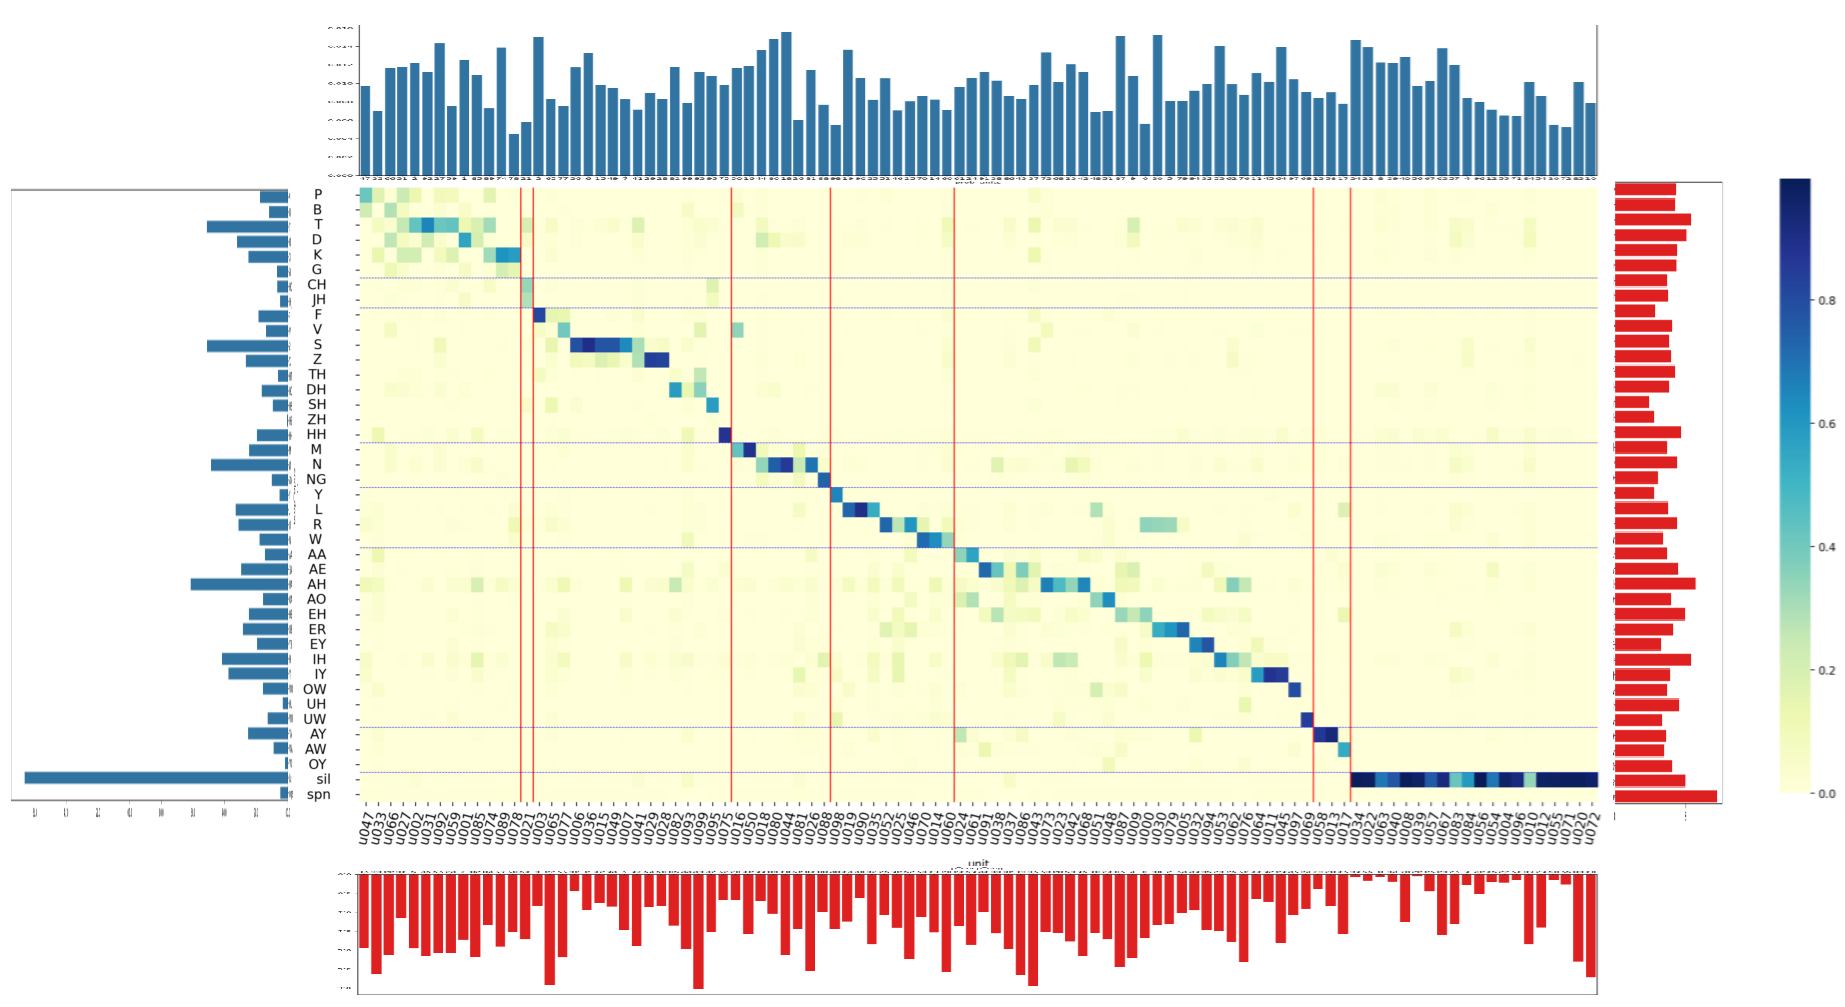
\includegraphics[width=1\linewidth]{figures/better__p_ph_given_un.png}
    \caption{HuBERT 100}
    \label{p_p_given_u-hub-100}
\end{figure}

  為了更直觀的了解模型離散單元與音素之間的對應關係,接下來的分析將把音素與單元的聯合分佈 \(p(p|u)\) 作圖呈現,如 \ref{p_p_given_u-hub-100} 所示。以下說明這張圖表的看法:

        橫軸是各單元,而縱軸是各音素,按照發音分組方式,輔音遵循國際音標的圖表排列,元音則按照 ARPABET (cite CMU Dict) 字母順序排列。由於離散單元編號本身並無特殊含義,因此當單元數太多時將省略。

        為了更好的看出各組別之間的關係,圖表上先將各組之間以橫線區分。按照語音學分組後,為了考慮單元之間的代表性,將每個單元都找出相對應最高機率的音素,接著將每個單元亦依照對應音素在縱軸的排列順序一一排列,若是遇到對應同一音素的兩種離散單元,則以 \(p(u|p) \) 由高至低排列。最後再橫軸上也以語音學分組區分。

        如此一來,便能夠呈現出一張由左上至右下的對應圖。這張圖在 (cite DinoSR) 等 paper 也有呈現。從圖中可以看出,用來編碼 sil 的 unit 其實佔據了不小的部分。
